\documentclass[11pt]{report}
\renewcommand{\baselinestretch}{1.5}


% Declaração dos pacotes
\usepackage[utf8]{inputenc}
\usepackage[T1]{fontenc}
\usepackage{graphicx}
\usepackage[portuguese]{babel}
\usepackage{graphicx}
\usepackage[affil-it]{authblk} % Usado para meter nome da escola
\usepackage{eurosym} % Usado para o €
\usepackage{url} % URL
\usepackage{listings}
\usepackage{color}
\definecolor{lightgray}{rgb}{.9,.9,.9}
\definecolor{darkgray}{rgb}{.4,.4,.4}
\definecolor{purple}{rgb}{0.65, 0.12, 0.82}

\lstdefinelanguage{JavaScript}
{
  keywords={typeof, new, true, false, catch, function, return, null, catch, switch, var, if, in, while, do, else, case, break},
  keywordstyle=\color{blue}\bfseries,
  ndkeywords={class, export, boolean, throw, implements, import, this},
  ndkeywordstyle=\color{darkgray}\bfseries,
  identifierstyle=\color{black},
  sensitive=false,
  comment=[l]{//},
  morecomment=[s]{/*}{*/},
  commentstyle=\color{purple}\ttfamily,
  stringstyle=\color{red}\ttfamily,
  morestring=[b]',
  morestring=[b]"
}

\lstset{
   language=JavaScript,
   backgroundcolor=\color{lightgray},
   extendedchars=true,
   basicstyle=\footnotesize\ttfamily,
   showstringspaces=false,
   showspaces=false,
   numbers=left,
   numberstyle=\footnotesize,
   numbersep=9pt,
   tabsize=2,
   breaklines=true,
   showtabs=false,
   captionpos=b
}






% CAPA
\title{\textbf{Exploração e desenvolvimento de um \textit{backend} e API WEB.}\\
		\large2º Trabalho prático de
		Multimédia e Tecnologia Web}
			
				
\author{ Kyrylo Yavorenko nº10355 \\ Rúben Guimarães nº11156}

\affil{Escola Superior de Tecnologia, IPCA \\
	Barcelos}	
	
		
\date{10 de Junho de 2018}


\begin{document}

\maketitle






% Introdução
\chapter*{Introdução}
\addcontentsline{toc}{chapter}{Introdução}

O trabalho prático abordado neste relatório foi desenvolvido no âmbito da unidade curricular Multimédia e Tecnologia Web do curso de Engenharia de Sistemas Informáticos, lecionada pelo docente Mickael da Costa. O docente desafiou os alunos a criar um projeto que aplicasse e experimenta-se metodologias e tecnologias de desenvolvimento de \textit{backend's} e API's WEB.

\clearpage






% Objectivos
\chapter*{Objectivos}
\addcontentsline{toc}{chapter}{Objectivos}

Os objetivos definidos para o projeto foram os seguintes:

\begin{itemize}
\item Desenvolvimento de modelo e um controlador tanto para os gif's como as categorias de gif's.
\item Criação de \textit{endpoint's} para:
	\subitem Devolver todos os gif's (GET),
	\subitem Devolver os gif's por categoria (GET),
	\subitem Devolver todas as categorias (GET),
	\subitem Criar um novo gif (POST),
	\subitem Criar uma nova categoria (POST),
	\subitem Editar uma categoria (PUT),
	\subitem Apagar um gif pelo ID (DELETE).
\item Botões dinâmicos consoante as categorias (frontend).
\item Obter os gif's pela categoria (frontend).
\item Permitir a adição de mais gif's e categorias(frontend).

\end{itemize}



\clearpage




% Desenvolvimento
\chapter*{Desenvolvimento}
\addcontentsline{toc}{chapter}{Desenvolvimento}


Começamos por estruturar as pastas e a criação de ficheiros de JavaScript para uma melhor organização do \textit{backend} tal como podemos verificar na imagem seguinte.

\begin{figure} [!h]
\centering
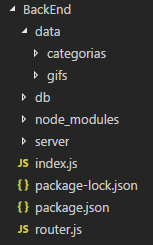
\includegraphics[width=25mm]{Prints_Trabalho/estrutura.png}
\caption{Estrutura do \textit{backend}.}
\label{Rotulo}
\end{figure}

De seguida criamos o controlador do projeto e os seus modelos para cada uma das categorias  e desenvolvemos o código necessário a estes, recorrendo a Node.JS. Para facilitar o nosso trabalho recorremos npm que é gestor de pacotes do JavaScrip  para instalar diversos pacotes que facilita-sem o nosso trabalho. Nos modelos tivemos que criar o \textit{squema} que ia ser usado para criar coleções dos dados em BSON no MongoDB. Nas imagens seguintes podes verificar o \textit{schema} criado.

\clearpage

\begin{figure} [h]
\centering
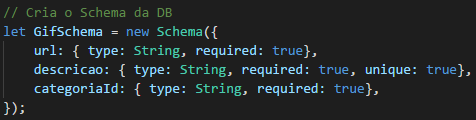
\includegraphics[width=\textwidth]{Prints_Trabalho/schemaGif.png}
\caption{\textit{Schema} dos gif's.}
\label{Rotulo}
\end{figure}

\begin{figure} [h]
\centering
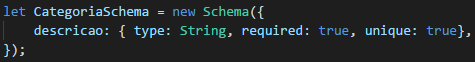
\includegraphics[width=\textwidth]{Prints_Trabalho/schemaCategorias.png}
\caption{Schema das categorias.}
\label{Rotulo}
\end{figure}

Para ligarmos a base de dados ao projeto recorremos ao pacote do npm mongoose tal como podemos ver na figura seguinte.

\medskip
\begin{lstlisting}[caption= Conexão a base de dados recorrendo ao mongoose.]
var config = { db: 'mongodb://localhost/dbWeb' };
mongoose.connect(config.db);
\end{lstlisting}

A maior parte do desenvolvimento foi a volta da criação dos \textit{endpoint's} necessários e o seu teste recorrendo ao software Postman. \\ Por fim adaptamos o \textit{frontend} do primeiro trabalho pratico, para usar a API desenvolvida e criamos duas novas paginas HTML com os seus respetivos ficheiros CSS e JavaScript para a criação e gif's e categorias.

% Conclução
\chapter*{Conclusão}
\addcontentsline{toc}{chapter}{Conclusão}

Este trabalho permitiu-se aplicar os conhecimentos adquiridos durante o desenrolar da unidade curricular de Multimédia e Tecnologia Web e explorar e desenvolver a criação de \textit{backend's} e API's. Uma das maiores dificuldade do trabalho foi perceber a lógica que os pedidos para API tinham que ser para funcionarem de forma correta. Outra dificuldade encontrada foi começar a usar pedidos AJAX para comunicar com a API, neste caso recorremos ao jQuery para facilitar. \\ Por fim achamos que o trabalho foi muito vantajoso tendo em conta que contactamos com uma grande numero de tecnologias orientadas ao desenvolvimento WEB  e permitiu o contacto com base de dados NoSQL.


\end{document}